\chapter{Исследовательская часть}

\section{Характеристики ЭВМ}

В листинге~\ref{lst:sysinfo} приведены характеристики ЭВМ и системы, использованных для проведения замеров времени выполнения реализаций алгоритмов.

\lstinputlisting[label=lst:sysinfo,caption=Частичный вывод команды systeminfo.exe --- характеристика ЭВМ]{listings/sysinfo.txt}
\clearpage

\section{Время выполнения алгоритмов}

Время работы алгоритмов измерялось с использованием функции
$clock$ библиотеки $ctime$.

Время умножения для каждого размера матриц считалось как среднее арифметическое из 100 повторений. На вход подавались квадратные матриц $A_{N \times N}$, заполненные числами $0$ до $N^2$.

В таблицах~\ref{tbl:time_even}~--~\ref{tbl:time_odd} приведены результатов времени умножения на различных размерах входных матриц.

\begin{table}[ht]
	\small
	\begin{center}
		\begin{threeparttable}
			\caption{Замер времени для чётных матриц размером от 2 до 1000}
			\label{tbl:time_even}
			\begin{tabular}{|r|r|r|r|}
				\hline
				& \multicolumn{3}{c|}{\bfseries Время, мс} \\
				\cline{2-4}
				\bfseries \makecell{Линейный размер} & \bfseries Классический & \bfseries Виноград & \bfseries Виноград (опт) \\
				\cline{2-4}
				\hline
				2 & 1.28 & 1.56 & 1.34 \\ 
				\hline 
				10 & 15.3 & 15.12 & 14.36 \\ 
				\hline 
				50 & 665.88 & 669.58 & 640.26 \\ 
				\hline 
				100 & 5273.9 & 5006.5 & 4992.96 \\ 
				\hline 
				200 & 41825.8 & 39184.7 & 39130.6 \\ 
				\hline 
				300 & 145676 & 138221 & 138054 \\ 
				\hline 
				400 & 355970 & 338145 & 337549 \\ 
				\hline 
				500 & 688205 & 653745 & 656862 \\ 
				\hline 
				750 & 2397640 & 2224810 & 2230590 \\ 
				\hline 
				1000 & 5876470 & 5460200 & 5455430 \\ 
				\hline
			\end{tabular}	
		\end{threeparttable}
	\end{center}
\end{table}

\begin{table}[ht]
	\small
	\begin{center}
		\begin{threeparttable}
			\caption{Замер времени для нечётных матриц размером от 1 до 1001}
			\label{tbl:time_odd}
			\begin{tabular}{|r|r|r|r|}
				\hline
				& \multicolumn{3}{c|}{\bfseries Время, мс} \\
				\cline{2-4}
				\bfseries \makecell{Линейный размер} & \bfseries Классический & \bfseries Виноград & \bfseries Виноград (опт) \\
				\cline{2-4}
				\hline
				1 & 0.86 & 1.14 & 1 \\ 
				\hline 
				11 & 13.92 & 14.38 & 13.42 \\ 
				\hline 
				51 & 714.8 & 708.2 & 687.58 \\ 
				\hline 
				101 & 5465.68 & 5209.92 & 5179.46 \\ 
				\hline 
				201 & 43404 & 40891.2 & 41091 \\ 
				\hline 
				301 & 152297 & 144547 & 144932 \\ 
				\hline 
				401 & 355688 & 338194 & 338850 \\ 
				\hline 
				501 & 698691 & 664296 & 664542 \\ 
				\hline 
				751 & 2426420 & 2249880 & 2263940 \\ 
				\hline 
				1001 & 5891340 & 5432400 & 5479120 \\
				\hline
			\end{tabular}	
		\end{threeparttable}
	\end{center}
\end{table}

\clearpage

На рисунках~\ref{img:graph_std_odd_vs_even}~--~\ref{img:graph_all_even} приведены графики времени умножения от размеров входных матриц.

\begin{figure}[H]
	%\centering
	\hspace*{-2cm}
	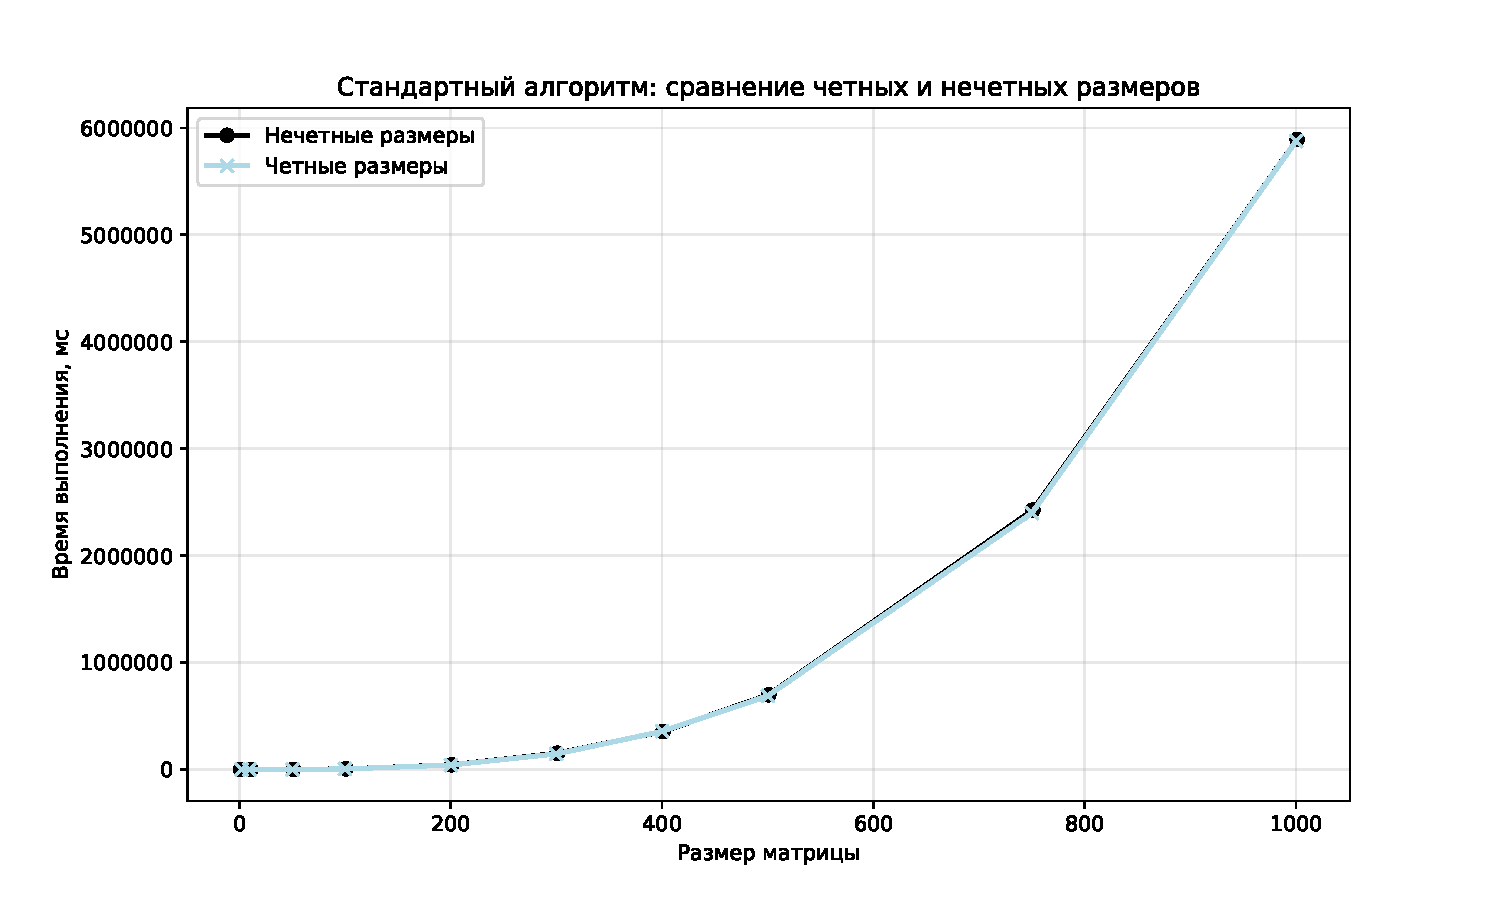
\includegraphics[scale=0.8]{images/std_odd_vs_even.pdf}
	\caption{Сравнение стандартного алгоритма на чётных и нечётных размерах}
	\label{img:graph_std_odd_vs_even}
\end{figure}
\clearpage

\begin{figure}[H]
	%\centering
	\hspace*{-2cm}
	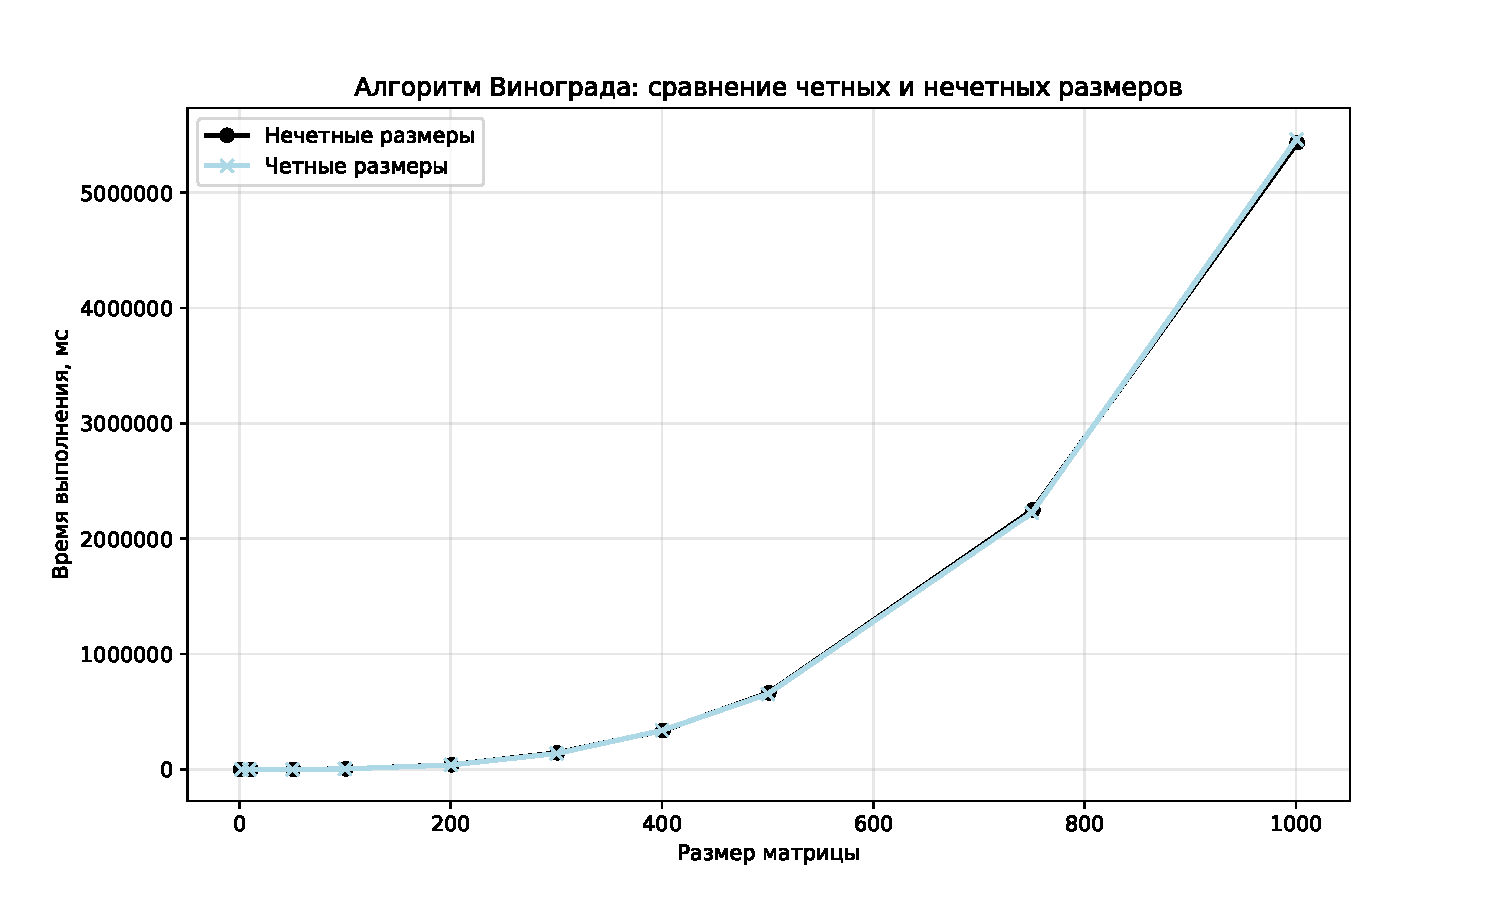
\includegraphics[scale=0.8]{images/winograd_odd_vs_even.pdf}
	\caption{Сравнение алгоритма Винограда на чётных и нечётных размерах}
	\label{img:graph_Win_odd_vs_even}
\end{figure}

\begin{figure}[H]
	%\centering
	\hspace*{-2cm}
	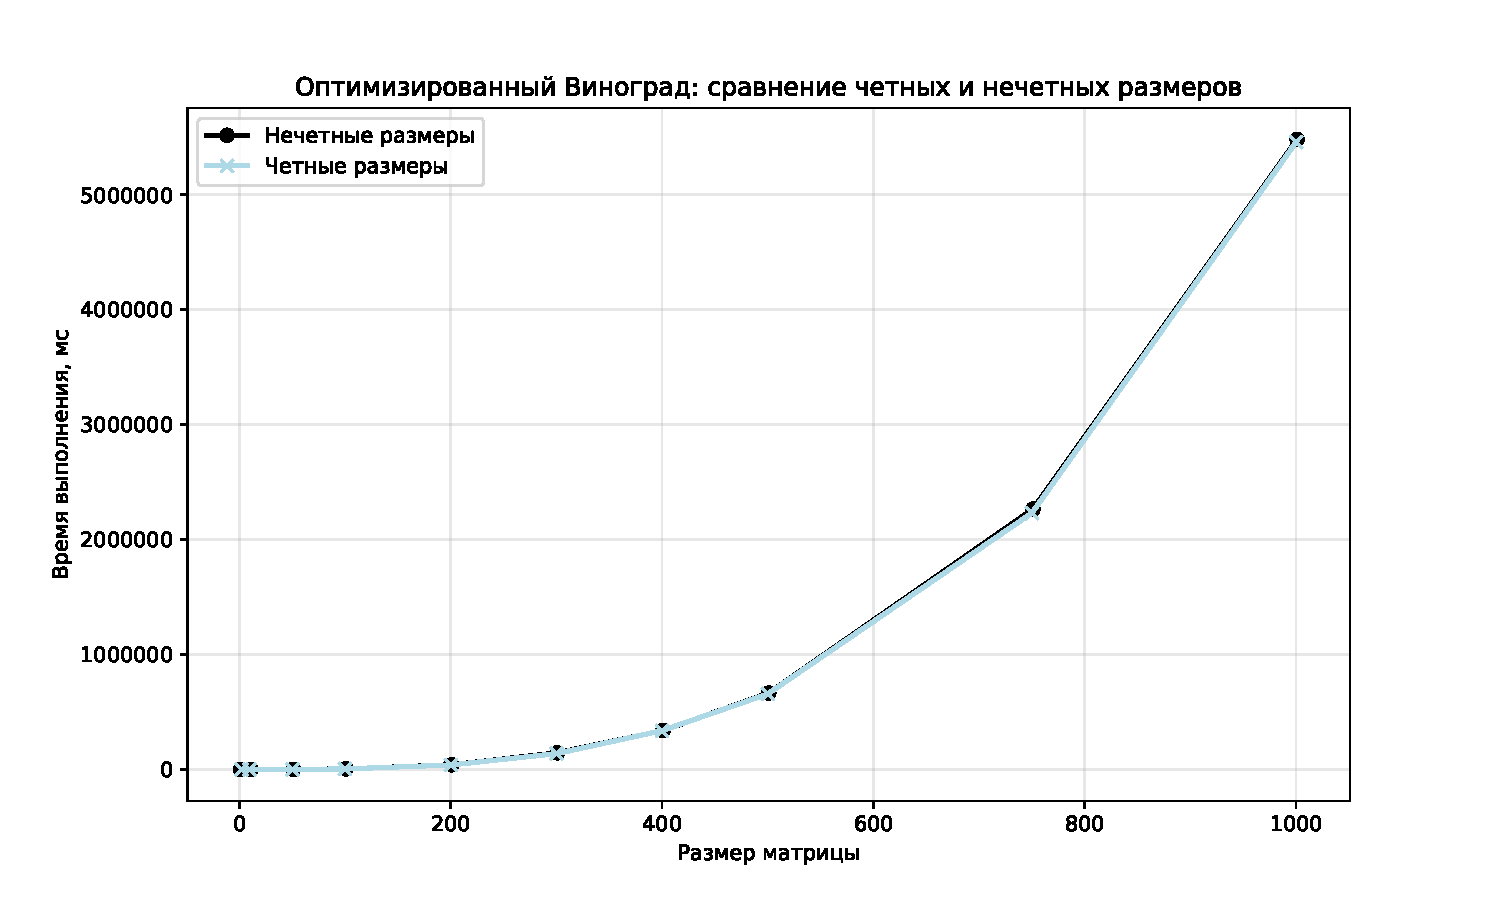
\includegraphics[scale=0.8]{images/optwinograd_odd_vs_even.pdf}
	\caption{Сравнение оптимизированного алгоритма Винограда на чётных и нечётных размерах}
	\label{img:graph_optWin_odd_vs_even}
\end{figure}
\clearpage

\begin{figure}[H]
	%\centering
	\hspace*{-2cm}
	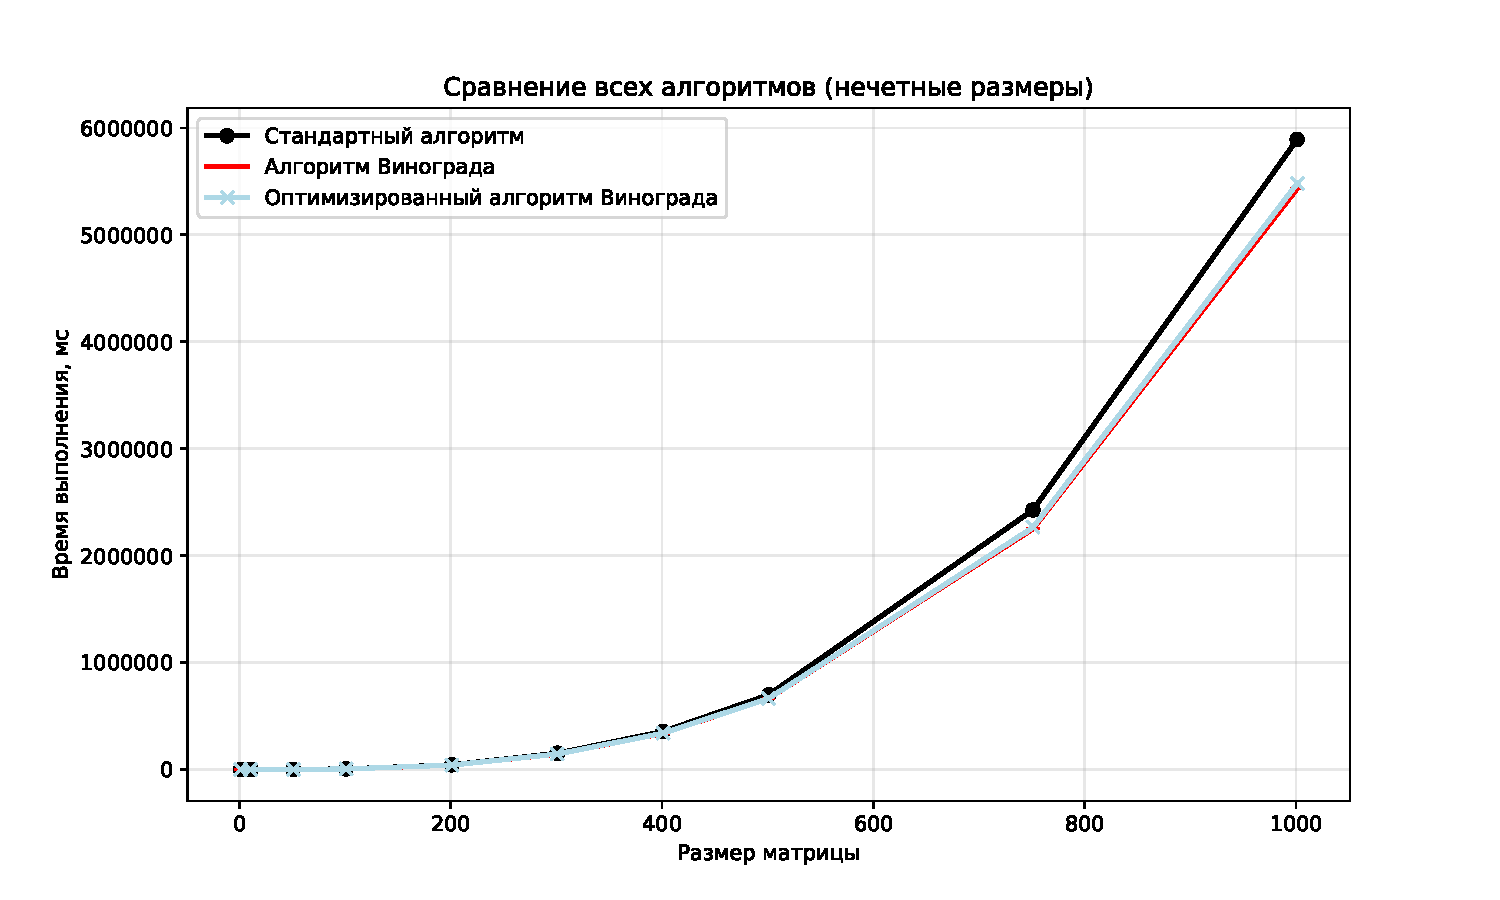
\includegraphics[scale=0.8]{images/all_algorithms_odd.pdf}
	\caption{Сравнение всех алгоритмов на чётных размерах}
	\label{img:graph_all_odd}
\end{figure}

\begin{figure}[H]
	%\centering
	\hspace*{-2cm}
	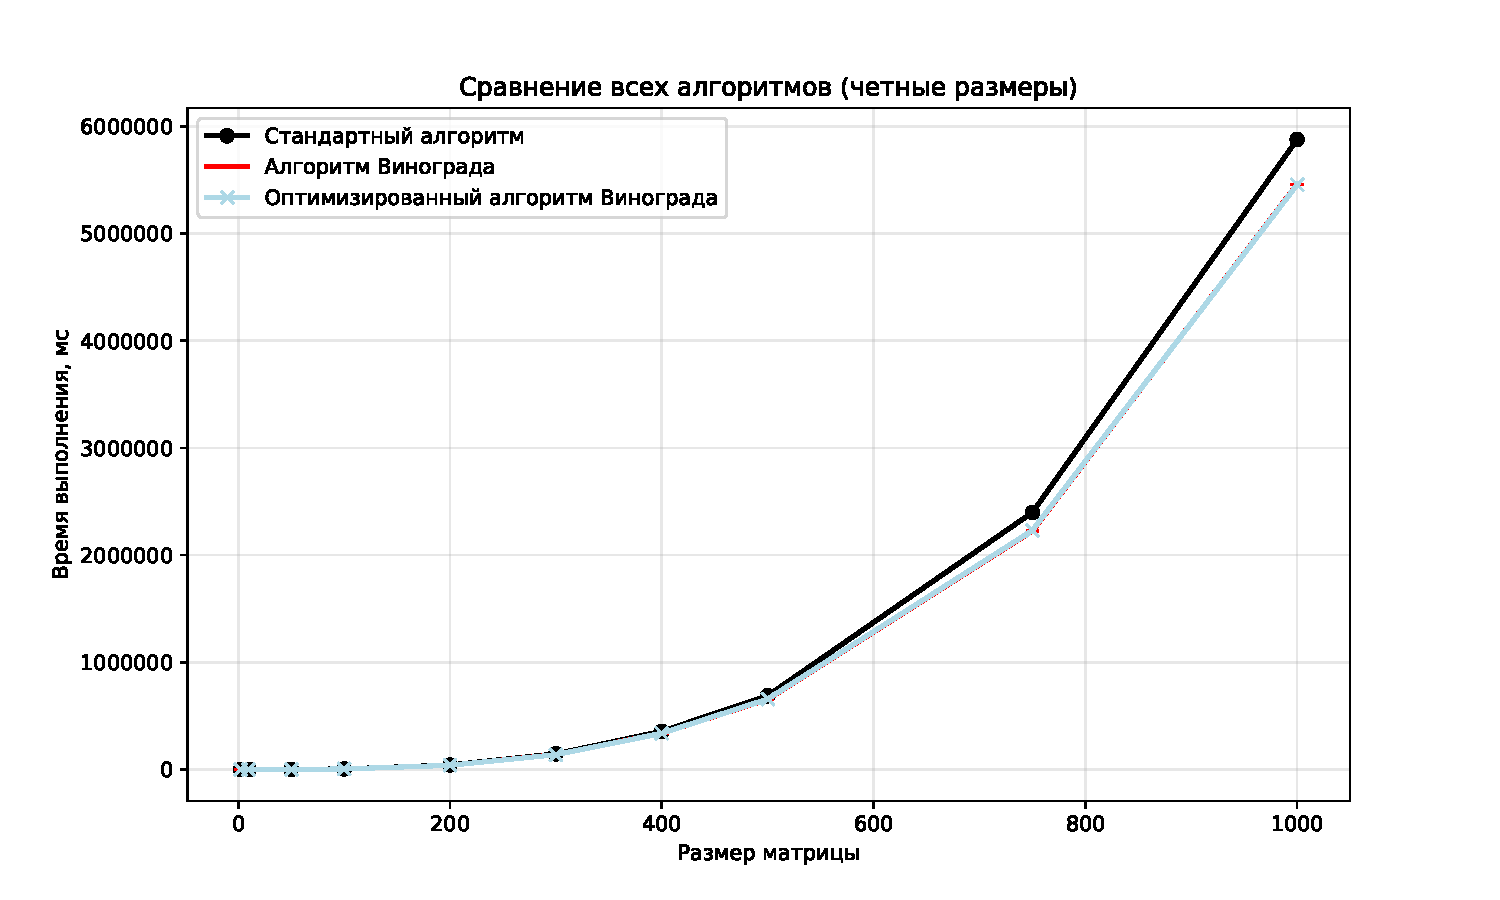
\includegraphics[scale=0.8]{images/all_algorithms_even.pdf}
	\caption{Сравнение всех алгоритмов на нечётных размерах}
	\label{img:graph_all_even}
\end{figure}
\clearpage

Приведённые данные показывают, что полученная реализация алгоритма винограда эффективнее реализации стандартного по времени выполнения (на $7\%$ при максимальном размере входных матриц). Разница между временем выполнения реализаций алгоритма Винограда и его оптимизированной версии оказалась минимальной.

Несущественной оказалась и разность времени работы описанных реализаций на близких по значению чётных и нечётных линейных размерах входных матриц (менее $1\%$ при линейном размере матриц более $200$)

%<цель исследования, на какой машине делали (указать ЦПУ, ОЗУ, ОС), желательно написать, как исследовали и при каких условиях; что получили в результате (таблицы + графики)>

\section*{Вывод}

В ходе анализа замеренного времени выполнения, было получено, что применять приведённую реализацию алгоритма Винограда имеет смысл при линейном размере входных матриц более $50$. Также было установлено, что дополнительные вычисления в реализации алгоритма Винограда при нечётном линейном размере входных матриц не вносят существенного вклада в итоговое время работы.

\clearpage
